% ============================================================
%  Aarhus University — Presentation Template
%  Light, minimal Beamer theme for project pitches,
%  results presentations, and status updates.
%  Sharp corners, high-contrast a11y palette.
% ============================================================
\documentclass[aspectratio=169, 12pt]{beamer}

% --- Encoding & language ---
\usepackage[utf8]{inputenc}
\usepackage[T1]{fontenc}
\usepackage[english]{babel}

% --- Clean sans-serif font ---
\usepackage{helvet}
\renewcommand{\familydefault}{\sfdefault}

% --- Graphics & figures ---
\usepackage{graphicx}
\graphicspath{{assets/}}
\usepackage{float}

% --- Math ---
\usepackage{amsmath}
\usepackage{amssymb}

% --- TikZ & plots ---
\usepackage{tikz}
\usepackage{pgfplots}
\pgfplotsset{compat=1.18}
\usepackage[european, straightvoltages]{circuitikz}

% --- Tables ---
\usepackage{booktabs}
\usepackage{tabularx}

% --- Code listings ---
\usepackage{listings}


% ============================================================
%  COLOUR PALETTE — light theme, a11y contrast on white
% ============================================================
%  All foreground colours pass WCAG AA (4.5:1) against white.
%  AU blue #003D73 = 7.9:1 contrast on white (AAA).
% ------------------------------------------------------------
\definecolor{aublue}{HTML}{003D73}       % AU primary — 7.9:1 on white
\definecolor{aubluelight}{HTML}{E0EBF5}  % AU blue tint — section bg
\definecolor{background}{HTML}{FFFFFF}   % pure white
\definecolor{foreground}{HTML}{09090B}   % zinc-950 — body text
\definecolor{muted}{HTML}{52525B}        % zinc-600 — 7.0:1 on white
\definecolor{border}{HTML}{E4E4E7}       % zinc-200 — lines, rules
\definecolor{cardbg}{HTML}{F4F4F5}       % zinc-100 — block backgrounds
\definecolor{codebg}{HTML}{F4F4F5}       % same as card
\definecolor{accentgreen}{HTML}{047857}  % emerald-700 — 5.3:1 on white
\definecolor{accentred}{HTML}{B91C1C}    % red-700 — 5.5:1 on white
\definecolor{accentamber}{HTML}{92400E}  % amber-800 — 6.5:1 on white


% ============================================================
%  BEAMER THEME — flat, no rounding, no shadows
% ============================================================
\usetheme{default}
\usecolortheme{default}
\setbeamercolor{background canvas}{bg=background}
\setbeamercolor{normal text}{fg=foreground}
\setbeamercolor{frametitle}{fg=foreground}
\setbeamercolor{structure}{fg=aublue}
\setbeamercolor{itemize item}{fg=aublue}
\setbeamercolor{itemize subitem}{fg=muted}
\setbeamercolor{enumerate item}{fg=aublue}
\setbeamercolor{block title}{fg=foreground, bg=cardbg}
\setbeamercolor{block body}{fg=foreground, bg=cardbg}
\setbeamercolor{alerted text}{fg=accentred}
\setbeamercolor{footline}{fg=muted}

% Remove all navigation chrome
\setbeamertemplate{navigation symbols}{}
\setbeamertemplate{headline}{}

% Wider content margins (default is ~10pt, too tight)
\setbeamersize{text margin left=24pt, text margin right=24pt}

% No rounded corners on blocks
\setbeamertemplate{blocks}[default]

% Bullet style — square, shadcn-like
\setbeamertemplate{itemize item}{\small\raise1pt\hbox{\rule{4pt}{4pt}}}
\setbeamertemplate{itemize subitem}{\scriptsize\raise1pt\hbox{\rule{3pt}{3pt}}}

% Enumerate style — bold AU blue numbers
\setbeamertemplate{enumerate item}{\normalsize\bfseries\color{aublue}\insertenumlabel.}

% Frame title formatting — tight spacing
\setbeamertemplate{frametitle}{%
  \vskip8pt
  {\Large\bfseries\insertframetitle\par}%
  \ifx\insertframesubtitle\empty\else
    \vskip1pt
    {\small\color{muted}\insertframesubtitle\par}%
  \fi
  \vskip-2pt
  {\color{border}\rule{\textwidth}{0.4pt}\par}%
  \vskip2pt
}

% Minimal footline: thin rule + slide number
\setbeamertemplate{footline}{%
  \vskip0pt
  {\color{border}\rule{\paperwidth}{0.4pt}}%
  \vskip4pt
  \hbox to \paperwidth{%
    \hfill
    \usebeamercolor[fg]{footline}%
    \scriptsize\insertframenumber\,/\,\inserttotalframenumber
    \hspace{24pt}%
  }%
  \vskip6pt
}


% ============================================================
%  CUSTOM COMMANDS
% ============================================================

% --- Section divider slide (large faded number + title + AU blue bar) ---
\newcommand{\sectionslide}[2]{%
  {%
    \setbeamertemplate{footline}{}%
    \begin{frame}[c]
      \begin{tikzpicture}[remember picture, overlay]
        \fill[aublue] (current page.north west) rectangle
          ([xshift=4pt]current page.south west);
      \end{tikzpicture}
      \centering
      {\fontsize{48}{52}\selectfont\bfseries\color{border}#1\par}
      \vskip4pt
      {\fontsize{24}{30}\selectfont\bfseries\color{aublue}#2\par}
      \vskip8pt
      {\color{aublue}\rule{5cm}{2pt}\par}
    \end{frame}
  }%
}

% --- Stat card (big number + label, sharp border, fixed height) ---
\newcommand{\stat}[2]{%
  \begin{minipage}[t]{0.30\textwidth}
    \centering
    \fboxsep=12pt
    \fcolorbox{border}{background}{%
      \parbox[c][3.2cm][c]{0.82\textwidth}{%
        \centering
        {\fontsize{28}{32}\selectfont\bfseries\color{aublue}#1\par}
        \vskip6pt
        {\small\color{muted}#2\par}
      }%
    }%
  \end{minipage}%
}

% --- Status labels (a11y-safe on white) ---
\newcommand{\done}{{\color{accentgreen}\rule{6pt}{6pt}\;\textbf{Done}}}
\newcommand{\ongoing}{{\color{accentamber}\rule{6pt}{6pt}\;\textbf{In Progress}}}
\newcommand{\planned}{{\color{muted}\rule{6pt}{6pt}\;\textbf{Planned}}}

% --- Callout box (sharp border, left accent bar, proper padding) ---
\newcommand{\callout}[2]{%
  \par\vskip4pt
  \noindent
  \begin{tikzpicture}
    \node[
      draw=border,
      fill=cardbg,
      inner xsep=14pt,
      inner ysep=8pt,
      minimum width=\textwidth,
      text width=\dimexpr\textwidth-28pt-0.8pt,
      font=\footnotesize,
      anchor=west,
    ] (box) {{\color{aublue}\bfseries #1}\\[2pt] #2};
    \fill[aublue] (box.north west) rectangle
      ([xshift=3pt]box.south west);
  \end{tikzpicture}
  \par
}

% --- Code listing defaults ---
\lstset{
  backgroundcolor=\color{codebg},
  basicstyle=\ttfamily\scriptsize\color{foreground},
  keywordstyle=\color{aublue}\bfseries,
  stringstyle=\color{accentgreen},
  commentstyle=\color{muted}\itshape,
  frame=single,
  framesep=6pt,
  rulecolor=\color{border},
  xleftmargin=8pt,
  xrightmargin=8pt,
  aboveskip=8pt,
  belowskip=8pt,
  breaklines=true,
  showstringspaces=false,
}


% ============================================================
%  METADATA (fill in per project)
% ============================================================
\newcommand{\presentationtitle}{Project Title}
\newcommand{\presentationsubtitle}{Subtitle or Course Name}
\newcommand{\authorA}{Author 1}
\newcommand{\authorB}{Author 2}
\newcommand{\supervisor}{Supervisor Name}
\newcommand{\department}{Department Name}

\title{\presentationtitle}
\subtitle{\presentationsubtitle}
\author{\authorA \and \authorB}
\institute{\department \\ Aarhus University}
\date{\today}


% ============================================================
\begin{document}

% --- Title slide ---
{
\setbeamertemplate{footline}{}
\begin{frame}[c]
  \centering
  \vskip8pt

  
\includegraphics[height=1cm]{aulogo_dk_var2_blaa}

  \vskip16pt

  {\fontsize{28}{34}\selectfont\bfseries\color{aublue} \presentationtitle \par}
  \vskip4pt
  {\normalsize\color{muted} \presentationsubtitle \par}

  \vskip12pt
  {\color{aublue}\rule{6cm}{1.5pt}\par}
  \vskip12pt

  {\small
    \authorA \quad\color{muted}{\textbar}\quad\color{foreground} \authorB
  \par}
  \vskip4pt
  {\scriptsize\color{muted}
    \department \quad\textbar\quad Aarhus University \quad\textbar\quad \today
  \par}
\end{frame}
}


% ============================================================
%  AGENDA
% ============================================================
\begin{frame}{Agenda}
  \vfill
  \begin{enumerate}
    \setlength{\itemsep}{10pt}
    \item Motivation \& Problem Statement
    \item Approach
    \item Key Results
    \item Status \& Timeline
    \item Next Steps
  \end{enumerate}
  \vfill
\end{frame}


% ============================================================
\sectionslide{01}{Motivation \& Problem Statement}
% ============================================================

\begin{frame}{The Problem}
  \framesubtitle{Why this matters}

  \begin{itemize}
    \setlength{\itemsep}{10pt}
    \item Current approaches to \textbf{X} are limited by \textbf{Y}
    \item This leads to a measurable gap in \textbf{Z}
    \item No existing solution addresses all three constraints simultaneously
  \end{itemize}

  \vfill

  \callout{Research question:}{%
    How can we improve X while maintaining constraints on Y and Z?}
\end{frame}


% ============================================================
\sectionslide{02}{Approach}
% ============================================================

\begin{frame}{Method Overview}
  \framesubtitle{Three-phase experimental design}

  \begin{columns}[T]
    \begin{column}{0.30\textwidth}
      \fboxsep=8pt
      \fcolorbox{border}{cardbg}{%
        \parbox[t][4cm]{\dimexpr\textwidth-20pt}{%
          \raggedright
          {\color{aublue}\bfseries Phase 1}\\[4pt]
          \textbf{Data Collection}\\[4pt]
          {\scriptsize\color{muted}
            Gather measurements under controlled conditions using apparatus A.}
        }%
      }
    \end{column}
    \begin{column}{0.30\textwidth}
      \fboxsep=8pt
      \fcolorbox{border}{cardbg}{%
        \parbox[t][4cm]{\dimexpr\textwidth-20pt}{%
          \raggedright
          {\color{aublue}\bfseries Phase 2}\\[4pt]
          \textbf{Modelling}\\[4pt]
          {\scriptsize\color{muted}
            Fit parametric models and validate against held-out data.}
        }%
      }
    \end{column}
    \begin{column}{0.30\textwidth}
      \fboxsep=8pt
      \fcolorbox{border}{cardbg}{%
        \parbox[t][4cm]{\dimexpr\textwidth-20pt}{%
          \raggedright
          {\color{aublue}\bfseries Phase 3}\\[4pt]
          \textbf{Evaluation}\\[4pt]
          {\scriptsize\color{muted}
            Compare with baselines and assess statistical significance.}
        }%
      }
    \end{column}
  \end{columns}
\end{frame}

\begin{frame}{System Diagram}
  \centering
  \vfill
  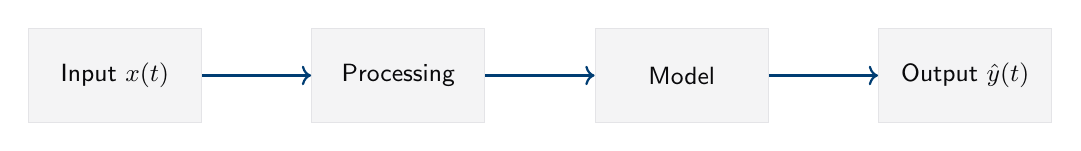
\begin{tikzpicture}[
    box/.style={draw=border, fill=cardbg, text=foreground,
                minimum width=2.2cm, minimum height=1.2cm, font=\small},
    arr/.style={->, thick, color=aublue}
  ]
    \node[box] (input) at (0,0) {Input $x(t)$};
    \node[box] (proc)  at (3.6,0) {Processing};
    \node[box] (model) at (7.2,0) {Model};
    \node[box] (out)   at (10.8,0) {Output $\hat{y}(t)$};

    \draw[arr] (input) -- (proc);
    \draw[arr] (proc)  -- (model);
    \draw[arr] (model) -- (out);
  \end{tikzpicture}
  \vfill
\end{frame}

\begin{frame}{Filter Design}
  \framesubtitle{Second-order Sallen-Key low-pass filter}

  \begin{columns}[c]
    \begin{column}{0.53\textwidth}
      \centering
      \begin{circuitikz}[scale=0.72, transform shape,
        every node/.style={font=\footnotesize}]
        % Input
        \draw (0,3) node[left]{$V_\text{in}$}
          to[R, l=$R_1$, o-, i>^=$i_1$] (2.5,3);
        % Second resistor
        \draw (2.5,3) to[R, l=$R_2$, i>^=$i_2$] (5,3);
        % Capacitor C1 from junction to ground
        \draw (2.5,3) to[C, l_=$C_1$, *-] (2.5,0.5)
          node[ground]{};
        % Junction to op-amp non-inverting input
        \draw (5,3) to[short, -*] (5.8,3);
        % Capacitor C2 from second junction to ground
        \draw (5.8,3) to[C, l=$C_2$] (5.8,0.5)
          node[ground]{};
        % Op-amp
        \draw (7,2.5) node[op amp, anchor=+](opamp){};
        \draw (5.8,3) to[short] (opamp.+);
        % Feedback: output to inverting input
        \draw (opamp.out) to[short, -*] ++(0.5,0)
          coordinate(out);
        \draw (out) to[short, -o] ++(0.5,0)
          node[right]{$V_\text{out}$};
        % Feedback wire
        \draw (opamp.-) to[short] ++(0,1.2)
          coordinate(fb);
        \draw (fb) -| (out);
        % Supply rails
        \draw (opamp.up) to[short] ++(0,0.4)
          node[above]{\scriptsize $+V_S$};
        \draw (opamp.down) to[short] ++(0,-0.4)
          node[below]{\scriptsize $-V_S$};
        % Voltage labels
        \draw[aublue, dashed, thin]
          (0,0.5) to[open, v_<=$V_\text{in}$] (0,3);
        \draw[aublue, dashed, thin]
          (9.8,0.5) to[open, v^<=$V_\text{out}$] (9.8,3);
        % Ground reference
        \draw (0,0.5) node[ground]{};
        \draw (9.8,0.5) node[ground]{};
      \end{circuitikz}
    \end{column}
    \hspace{8pt}
    \begin{column}{0.42\textwidth}
      \raggedright
      {\color{aublue}\bfseries Transfer function}\\[3pt]
      {\footnotesize $H(s) = \dfrac{1}{1 + s(R_1\!+\!R_2)C_2 + s^2 R_1 R_2 C_1 C_2}$}

      \vskip6pt
      {\color{aublue}\bfseries Design values}\\[3pt]
      \renewcommand{\arraystretch}{1.05}
      {\footnotesize
      \begin{tabular}{@{}l l@{}}
        $R_1, R_2$  & $10\;\text{k}\Omega$ \\
        $C_1, C_2$  & $1\;\text{nF}$ \\
        $f_c$       & $15.9\;\text{kHz}$ \\
        $Q$         & $0.5$ \\
      \end{tabular}}

      \vskip6pt
      {\scriptsize\color{muted}
        Unity gain, Butterworth at $Q\!=\!0.707$,
        $-40\;\text{dB/dec}$ above $f_c$.}
    \end{column}
  \end{columns}
\end{frame}


% ============================================================
\sectionslide{03}{Key Results}
% ============================================================

\begin{frame}{Results at a Glance}
  \centering
  \vfill

  \stat{94\%}{Model Accuracy ($R^2$)}
  \hfill
  \stat{12.1\,ms}{Time Constant ($\tau$)}
  \hfill
  \stat{3$\times$}{Speedup vs Baseline}

  \vskip20pt

  {\small\color{muted}
    Averaged across $n = 3$ independent trials under identical conditions.}
  \vfill
\end{frame}

\begin{frame}{Measured vs.\ Predicted}
  \centering
  \vskip2pt
  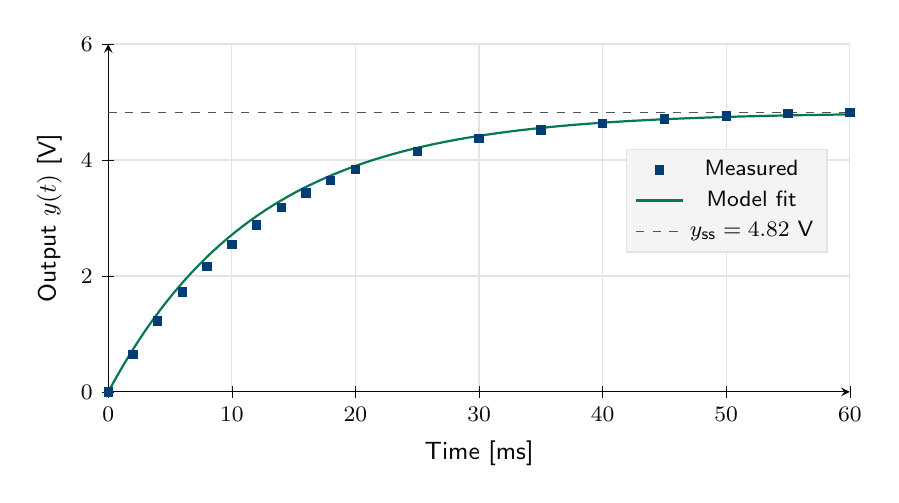
\begin{tikzpicture}
    \begin{axis}[
      width=11cm, height=6cm,
      xlabel={Time [ms]},
      ylabel={Output $y(t)$ [V]},
      xmin=0, xmax=60,
      ymin=0, ymax=6,
      grid=major,
      grid style={draw=border},
      axis lines=left,
      axis line style={foreground},
      tick style={foreground},
      ticklabel style={color=foreground, font=\footnotesize},
      label style={color=foreground, font=\small},
      legend style={
        at={(0.97,0.55)},
        anchor=east,
        fill=cardbg,
        draw=border,
        text=foreground,
        font=\footnotesize,
      },
    ]
    \addplot[only marks, mark=square*, aublue, mark size=1.5pt]
      coordinates {
        (0,0) (2,0.65) (4,1.22) (6,1.72) (8,2.16) (10,2.54)
        (12,2.88) (14,3.18) (16,3.43) (18,3.65) (20,3.84)
        (25,4.15) (30,4.37) (35,4.52) (40,4.63) (45,4.71)
        (50,4.76) (55,4.80) (60,4.82)
      };
    \addlegendentry{Measured}

    \addplot[accentgreen, thick, domain=0:60, samples=100]
      {4.82 * (1 - exp(-x/12.1))};
    \addlegendentry{Model fit}

    \addplot[dashed, muted, thin]
      coordinates {(0,4.82)(60,4.82)};
    \addlegendentry{$y_\text{ss} = 4.82$ V}
    \end{axis}
  \end{tikzpicture}
\end{frame}

\begin{frame}{Summary of Findings}
  \framesubtitle{Three independent trials}

  \vfill
  \renewcommand{\arraystretch}{1.4}
  \begin{tabularx}{\textwidth}{X r r r}
    \textbf{Trial}
      & $y_\text{ss}$ \textbf{[V]}
      & $\tau$ \textbf{[ms]}
      & $R^2$ \\[2pt]
    Trial 1 & 4.78 & 12.3 & 0.993 \\
    Trial 2 & 4.85 & 11.8 & 0.991 \\
    Trial 3 & 4.82 & 12.1 & 0.995 \\[2pt]
    \textbf{Mean} & \textbf{4.82} & \textbf{12.1} & \textbf{0.993} \\
  \end{tabularx}

  \vfill

  \callout{Key takeaway:}{%
    All trials achieved $R^2 > 0.99$, confirming the first-order model
    accurately captures the system dynamics.}
\end{frame}


% ============================================================
\sectionslide{04}{Status \& Timeline}
% ============================================================

\begin{frame}{Project Status}
  \framesubtitle{Updated \today}

  \vfill
  \renewcommand{\arraystretch}{1.4}
  \begin{tabularx}{\textwidth}{X l l}
    \textbf{Milestone} &
    \textbf{Deadline} &
    \textbf{Status} \\[2pt]
    Literature review        & Week 4  & \done \\
    Data collection          & Week 8  & \done \\
    Model implementation     & Week 10 & \ongoing \\
    Validation \& testing    & Week 12 & \planned \\
    Report writing           & Week 14 & \planned \\
    Final presentation       & Week 16 & \planned \\
  \end{tabularx}
  \vfill
\end{frame}


% ============================================================
\sectionslide{05}{Next Steps}
% ============================================================

\begin{frame}{What's Next}
  \begin{itemize}
    \setlength{\itemsep}{12pt}
    \item Complete parameter sweep across remaining conditions
    \item Run frequency-domain characterisation (Bode analysis)
    \item Draft results and discussion sections of the report
    \item Prepare for final review with \supervisor
  \end{itemize}

  \vfill

  \callout{Key deadline:}{%
    Validation complete by Week 12 to stay on track.}
\end{frame}


% ============================================================
%  CLOSING SLIDE
% ============================================================
{
\setbeamertemplate{footline}{}
\begin{frame}[c]
  \centering

  {\fontsize{32}{38}\selectfont\bfseries\color{aublue} Thank You\par}
  \vskip6pt
  {\normalsize Questions?\par}

  \vskip20pt

  
\includegraphics[height=0.9cm]{aulogo_dk_var2_blaa}

  \vskip14pt

  {\scriptsize\color{muted}
    \authorA \quad\textbar\quad \authorB
    \quad\textbar\quad \department
    \quad\textbar\quad Aarhus University
  \par}
  \vskip4pt
  {\scriptsize\color{muted}
    author@post.au.dk
  \par}
\end{frame}
}


% ============================================================
% REMINDER: GAI Declaration (Generativ Kunstig Intelligens)
% ============================================================
% If you used GAI tools (e.g. ChatGPT, Copilot, Claude) to
% prepare this presentation, AU requires a separate GAI
% declaration submitted in WISEflow. See declaration.tex.
% ============================================================

\end{document}
